\subsection{Pöschl-Tellerův potenciál}
    Částice o hmotnosti $M$ se pohybuje v jednorozměrné konečně hluboké potenciálové jámě popsané funkcí
    \begin{align}
        V(x)&=\frac{V_{0}}{\cosh^{2}\frac{x}{d}},
    \end{align}
    kde $V_{0}<0$ udává hloubku jámy a $d>0$ její šířku (viz obrázek~\ref{fig:PoschlTeller}).
    Určete energetické spektrum.

\begin{solution}
    Prvním krokem bude převést Schrödingerovu rovnici pro vlnovou funkci $\psi=\psi(x)$,
    \begin{equation}
        \label{eq:PoschlTellerEquation}
        -\frac{\hbar^{2}}{2M}\psi_{xx}+\left[V(x)-E\right]\psi=0
    \end{equation}
    ($\psi_{x}\equiv\d\psi/\d x$ je zkrácený symbol pro derivaci), do tvaru rovnice pro hypergeometrickou funkci~\eqref{eq:HypergeometricEquation}.
    K~tomu je nutné provést postupně několik substitucí.

    \begin{enumerate}
    \item
        Předně je výhodné přejít k bezrozměrným veličinám pro souřadnici
        \begin{equation}
            \xi\equiv\frac{x}{d}
        \end{equation}
        a energii
        \begin{align}
            \epsilon&\equiv-\frac{\hbar^{2}}{2Md^{2}},
            &e&\equiv\frac{E}{\epsilon}>0,
            &v_{0}&\equiv\frac{V_{0}}{\epsilon}>0,
            &v(\xi)&\equiv\frac{V(\xi)}{\epsilon}=\frac{v_{0}}{\cosh^{2}\xi}
        \end{align}
        (faktor $\epsilon$ byl zvolen záporný, aby parametry $e$ a $v_{0}$ byly kladné)
        ve kterých Schrödingerova rovnice~\eqref{eq:PoschlTellerEquation} zní
        \begin{equation}
            \label{eq:PoschlTellerEquationXi}
            \psi_{\xi\xi}+\left[v(\xi)-e\right]\psi=0.
        \end{equation}

    \item
        Vlnovou funkci budeme hledat ve tvaru
        \begin{equation}
            \psi(\xi)=u(\xi)\cosh^{-\alpha}\xi,
        \end{equation}
        kde $\alpha>0$ je prozatím volný parametr, jehož hodnota bude zafixována později.
        Faktor $\cosh^{-\alpha}\xi$ zajistí správnou asymptotiku vlnové funkce pro $x\rightarrow\pm\infty$.
        
        První a druhá derivace funkce $\psi(\xi)$ jsou
        \begin{subequations}
            \begin{align}
                \psi_{\xi}&=u_{\xi}\,c^{-\alpha}-\alpha\,u\,c^{-\alpha-1}s,\\
                \psi_{\xi\xi}&=u_{\xi\xi}\,c^{-\alpha}-2\alpha\,u_{\xi}\,c^{-\alpha-1}s+\alpha(\alpha+1)\,u\,c^{-\alpha-2}\underbrace{s^{2}}_{c^{2}-1}-\alpha\,u\,c^{-\alpha-1}c\nonumber\\
                &=u_{\xi\xi}\,c^{-\alpha}-2\alpha\,u_{\xi}\,c^{-\alpha-1}s+\alpha^{2}\,u\,c^{-\alpha}-\alpha(\alpha+1)\,u\,c^{-\alpha-2},
            \end{align}            
        \end{subequations}
        kde se pro zestručnění zápisu používají zkratky pro hyperbolické funkce
        \begin{align}
            s&\equiv\sinh\xi,
            &c&\equiv\cosh\xi.
        \end{align}
        Dosazení do~\eqref{eq:PoschlTellerEquationXi} a vynásobení rovnice výrazem $c^{\alpha}$ vede na Schödingerovu rovnici pro funkci $u(\xi)$,
        \begin{equation}
            \label{eq:PoschlTellerEquationU}
            u_{\xi\xi}-2\alpha\,u_{\xi}\,\frac{s}{c}+\left(\alpha^{2}-e\right)u-\left[\alpha(\alpha+1)-v_{0}\right]u\,c^{-2}=0.
        \end{equation}

    \item
        Poslední člen Schrödingerovy rovnice lze vynulovat vhodnou volbou do této chvíle volného parametru $\alpha$.
        Podmínka získaná řešením kvadratické rovnice
        \begin{equation}
            \alpha(\alpha+1)-v_{0}=0
        \end{equation}
        je
        \begin{equation}
            \label{eq:PoschlTellerAlpha}
            \alpha=\frac{1}{2}\left(-1\pm\sqrt{1+4v_{0}}\right).
        \end{equation}
        Pro dobré asymptotické chování vlnové funkce $\psi$ je nutné, aby $\alpha>0$, což splňuje pouze kořen se znaménkem $+$.

        Schrödingerova rovnice~\eqref{eq:PoschlTellerEquationU} pro toto konkrétní $\alpha$ zní
        \begin{equation}
            u_{\xi\xi}+2\alpha\,u_{\xi}\,\frac{s}{c}+\left(\alpha^{2}-e\right)u=0.
        \end{equation}

    \item
        Poslední substitucí je zavedení nové nezávisle proměnné
        \begin{equation}
            z\equiv-\sinh^{2}\xi.
        \end{equation}
        Platí
        \begin{subequations}
            \begin{align}
                u_{\xi}&\equiv\derivative{u}{\xi}=\derivative{u}{z}\derivative{z}{\xi}=u_{z}z_{\xi},\\
                u_{\xi\xi}&\equiv\derivative[2]{u}{\xi}=\derivative[2]{u}{z}\left(\derivative{z}{\xi}\right)^{2}+\derivative{u}{z}\derivative[2]{z}{\xi}=u_{zz}z_{\xi}^{2}+u_{z}z_{\xi\xi}
            \end{align}
        \end{subequations}
        a dále pro substituční funkci
        \begin{subequations}
            \begin{align}
                z_{\xi}&=-2sc,\\
                z_{\xi\xi}&=-2(c^{2}+s^{2}).
            \end{align}
        \end{subequations}
        Dosazení do Schödingerovy rovnice dá
        \begin{equation}
            4\underbrace{s^{2}}_{-z}\underbrace{c^{2}}_{1-z}u_{zz}-2\left(c^{2}+s^{2}\right)u_{z}+4\alpha\,s^{2}\,u_{z}+\left(\alpha^{2}-e\right)u=0
        \end{equation}
        a po vynásobení obou stran výrazem $-\frac{1}{4}$ a úpravě
        \begin{equation}
            \label{eq:PoschlTellerEquationFinal}
            z(1-z)u_{zz}+\left[\frac{1}{2}-(1-\alpha)z\right]u_{z}-\frac{1}{4}\left(\alpha^{2}-e\right)u=0.
        \end{equation}

    \item 
        Finální rovnice~\eqref{eq:PoschlTellerEquationFinal} má tvar rovnice pro hypergeometrické funkce~\eqref{eq:HypergeometricEquation} s hodnotami parametrů $(a,b,c)$ danými vztahy
        \begin{subequations}
            \begin{align}
                a+b+1&=1-\alpha,\\
                ab&=\frac{1}{4}\left(\alpha^{2}-e\right),\\
                c&=\frac{1}{2}.
            \end{align}                
        \end{subequations}
        Řešení prvních dvou rovnic dá\sfootnote{
            Druhé možné řešení této soustavy rovnic je
            \begin{subequations}
                \begin{align}
                    a&=\frac{1}{2}\left(-\alpha-\sqrt{e}\right),\\
                    b&=\frac{1}{2}\left(-\alpha+\sqrt{e}\right),
                \end{align}                    
            \end{subequations}
            které však díky symetrii hypergeometrických funkcí vůči záměně prvního a druhého argumentu, $\2F1{a}{b}{c}{z}=\2F1{b}{a}{c}{z}$ vede na totožné řešení diferenciální rovnice~\eqref{eq:PoschlTellerEquationFinal}.
        }
        \begin{subequations}
            \begin{align}
                a&=\frac{1}{2}\left(-\alpha+\sqrt{e}\right),\\
                b&=\frac{1}{2}\left(-\alpha-\sqrt{e}\right).
            \end{align}                
        \end{subequations}

    \item
        Schrödingerova rovnice~\eqref{eq:PoschlTellerEquationFinal} má dvě lineárně nezávislá řešení daná hypergeometrickými funkcemi
        \begin{align}
            u_{1}(z)&=\2F1{\frac{1}{2}\left(-\alpha+\sqrt{e}\right)}{\frac{1}{2}\left(-\alpha-\sqrt{e}\right)}{\frac{1}{2}}{z},\\
            u_{2}(z)&=\sqrt{z}\2F1{\frac{1}{2}\left(-\alpha+\sqrt{e}+1\right)}{\frac{1}{2}\left(-\alpha-\sqrt{e}+1\right)}{\frac{3}{2}}{z}.
        \end{align}

    \item
        Vlnová funkce musí vymizet v asymptotické oblasti $x\rightarrow\pm\infty$ ($z\rightarrow-\infty$).
        K prozkoumání chování v nekonečnu se aplikuje vztah~\eqref{eq:2F1Asymptotic}.
        Za předpokladu
        \begin{equation}
            a-b\notin\mathbb{Z}\quad\Leftrightarrow\quad\sqrt{e}\notin\mathbb{Z}
        \end{equation}
        lze vztah použít.
        Limita $\xi\rightarrow\infty$
        \begin{align}
            \psi_{1}(\xi)\rightarrow
                &\cosh^{-\alpha}\xi\left\{
                    \underbrace{\frac{\Gamma\left(\frac{1}{2}\right)\Gamma\left(-\sqrt{e}\right)}{\Gamma\left[\frac{1}{2}\left(-\alpha-\sqrt{e}\right)\right]\Gamma\left[\frac{1}{2}\left(1+\alpha-\sqrt{e}\right)\right]}\sinh^{-\left(-\alpha+\sqrt{e}\right)}\xi}_{\gamma_{1}}\right.\nonumber\\
                &\qquad+\left.\underbrace{\frac{\Gamma\left(\frac{1}{2}\right)\Gamma\left(\sqrt{e}\right)}{\Gamma\left[\frac{1}{2}\left(-\alpha+\sqrt{e}\right)\right]\Gamma\left[\frac{1}{2}\left(1+\alpha+\sqrt{e}\right)\right]}\sinh^{-\left(-\alpha-\sqrt{e}\right)}\xi}_{\gamma_{2}}\right\}\nonumber\\
                &\sim\frac{1}{2}\e^{-\alpha\xi}\left\{\frac{\gamma_{1}}{2}\e^{\left(\alpha-\sqrt{e}\right)\xi}
                +\frac{\gamma_{2}}{2}\e^{\left(\alpha+\sqrt{e}\right)\xi}\right\}\nonumber\\
                &\sim\frac{\gamma_{1}}{4}\e^{-\sqrt{e}\,\xi}+\frac{\gamma_{2}}{4}\e^{\sqrt{e}\,\xi}\rightarrow\infty
        \end{align}
        diverguje.
        Řešení $u_{1}$ je tedy nutné omezit na polynom podmínkou $a=-n$ nebo $b=-n$, $n\in\mathbb{N}_{0}$.
        Tyto podmínky vedou na
        \begin{subequations}
            \begin{align}
                \frac{1}{2}\left(-\alpha+\sqrt{e}\right)&=-n &&\longrightarrow &\alpha&=2n+\sqrt{e} \\
                \frac{1}{2}\left(-\alpha-\sqrt{e}\right)&=-n &&\longrightarrow &\alpha&=2n-\sqrt{e}.
            \end{align}                
        \end{subequations}
        Jelikož $e>0$, vede druhá podmínka na divergující řešení s $\alpha<0$.
        První podmínka dá možné diskrétní energetické hladiny (kvantovací podmínka)
        \begin{align}
            \sqrt{e_{1,n}}&=\alpha-2n\nonumber\\
            e_{1,n}&=\left(\alpha-2n\right)^{2}\nonumber\\
            E_{1,n}&=-\frac{\hbar^{2}}{8Md^{2}}\left[\sqrt{1-\frac{8MV_{0}d^{2}}{\hbar^{2}}}-1-4n\right]^{2},
        \end{align}
        přičemž první řádek vede na dodatečné omezení počtu kvantových hladin: pravá strana totiž musí být kladná, tj. musí být splněno
        \begin{equation}
            n<\frac{\alpha}{2}=\frac{1}{4}\left[\sqrt{1-\frac{8MV_{0}d^{2}}{\hbar^{2}}}-1\right]
        \end{equation}

        Pro druhé řešení $\psi_{2}$ se postupuje zcela analogicky.
        Kvantovací podmínka vyjde
        \begin{equation}
            \alpha=2n+\sqrt{e}+1,
        \end{equation}
        takže
        \begin{equation}
            E_{2,n}=-\frac{\hbar^{2}}{8Md^{2}}\left[\sqrt{1-\frac{8MV_{0}d^{2}}{\hbar^{2}}}-3-4n\right]^{2}.
        \end{equation}
        a $n$ je mezeno shora nerovností
        \begin{equation}
            n<\frac{\alpha}{2}-\frac{1}{2}=\frac{1}{4}\left[\sqrt{1-\frac{8MV_{0}d^{2}}{\hbar^{2}}}-3\right]
        \end{equation}

        Obě řešení $E_{1,n}$ a $E_{2,n}$ lze zapsat jedním výrazem
        \begin{equation}
            \important{E_{n}=-\frac{\hbar^{2}}{8Md^{2}}\left[\sqrt{1-\frac{8MV_{0}d^{2}}{\hbar^{2}}}-(2n+1)\right]^{2}}
        \end{equation}
        za podmínky
        \begin{equation}
            n<\frac{1}{2}\left[\sqrt{1-\frac{8MV_{0}d^{2}}{\hbar^{2}}}-1\right].
        \end{equation}
        Odpovídající (nenormalizované) vlnové funkce jsou
        \begin{equation}
            \psi_{n}(x)=\left\{
                \begin{array}{ll}
                    \cosh^{-\alpha}\left(\frac{x}{d}\right)\2F1{-\frac{n}{2}}{\frac{n}{2}-\alpha}{\frac{1}{2}}{-\sinh^{2}\left(\frac{x}{d}\right)}, & n\ \text{liché,}\\           
                    -\cosh^{-\alpha}\left(\frac{x}{d}\right)\sinh\left(\frac{x}{d}\right)\2F1{-\frac{n+1}{2}}{\frac{n+1}{2}-\alpha}{\frac{3}{2}}{-\sinh^{2}\left(\frac{x}{d}\right)},& n\ \text{sudé,}
                \end{array}\right.
        \end{equation}
        kde $\alpha$ je dáno vztahem~\eqref{eq:PoschlTellerAlpha}.

		\begin{figure}[!htbp]
			\centering
			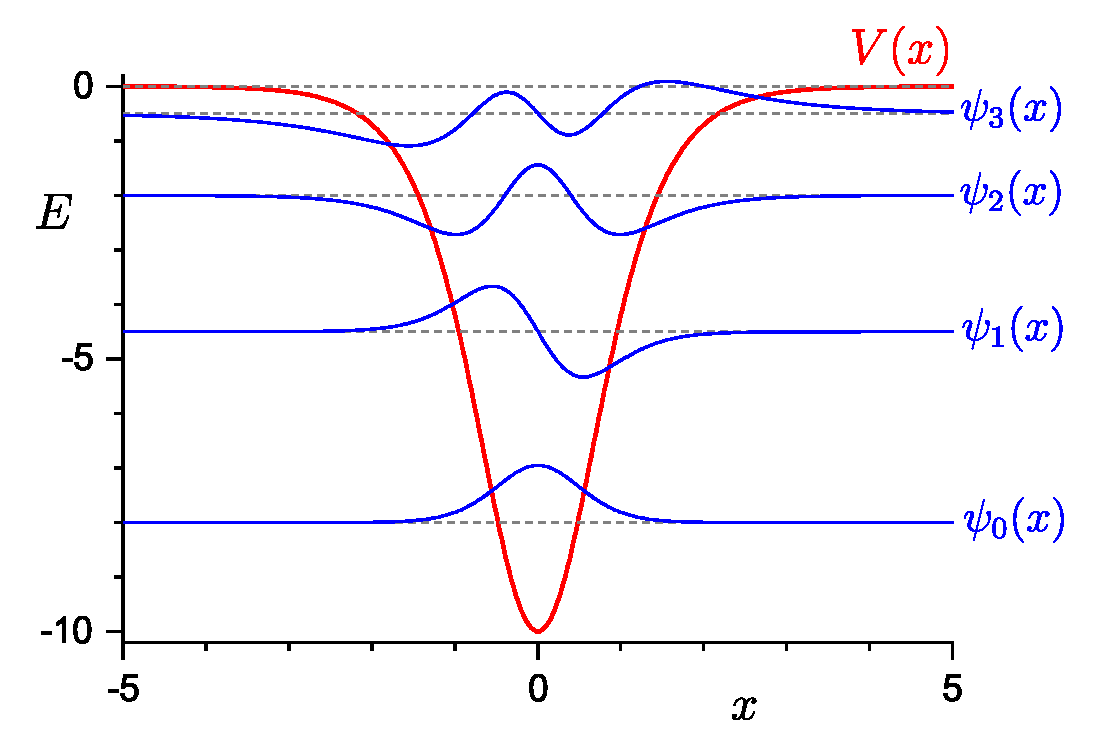
\epsfig{file=figures/PoschlTeller.eps,width=0.8\linewidth}
			\caption{
                Pöschl-Tellerův potenciál a všechny diskrétní energetické hladiny, které systém pro $M=\hbar=1$ a $V=10$ má.
                Vlnové funkce jsou normované a posunuté na místo odpovídající energetické hladiny.
                Hladina $\psi_{4}$ s energií $E=0$ již není normalizovatelná.
			}
			\label{fig:PoschlTeller}
        \end{figure}			
        
        Několik hladin a příslušné vlnové funkce jsou zobrazeny na obrázku~\ref{fig:PoschlTeller}.

    \end{enumerate}
\end{solution}
